\section{Proximal Policy Optimization}

\subsection{PPO introduced by OpenAI}
When performing the policy gradient update, each step one needs to sample the trajectories of the environment (since after one update on the policy $\pi_\theta$, the trajectory becomes obsolete. How can we address the sample efficiency issue? Importance sampling comes to rescue.


Consider the gradient estimator function, where $\hat A_\phi$ is any "good" estimate of the advantage\footnote{As the subscripts suggests, the definition of $\hat A_\phi$ usually rely on the value function $V^{\pi}_{\phi}$. }.

\begin{align*}
   \widetilde{\grad_{\theta}\Jcal}(\theta)
   & =\Embb_{\tau\sim \pi_{\theta}}\left[ \sum_{t=0}^{T-1} \hat A_\phi(s_t,a_t)\grad_{\theta}\log\pi_{\theta}(a_t|s_t)\right] 
   =\Embb_{\tau\sim \pi_{\theta_{\text{old}}}}\left[ \sum_{t=0}^{T-1}\frac{\pi_{\theta}(a_t|s_t)}{\pi_{\theta_{\text{old}}}(a_t|s_t)} \hat A_\phi(s_t,a_t)\grad_{\theta}\log\pi_{\theta}(a_t|s_t)\right] \\
   & = \Embb_{\tau\sim \pi_{\theta_{\text{old}}}}\left[ \sum_{t=0}^{T-1}\frac{1}{\pi_{\theta_{\text{old}}}(a_t|s_t)} \hat A_\phi(s_t,a_t)\grad_{\theta}\pi_{\theta}(a_t|s_t)\right].
\end{align*}
The corresponding objective function can be written as 
\begin{align*}
   \Jcal_{\text{advantage}}(\theta):= \Embb_{\tau\sim \pi_{\theta_{\text{old}}}}\left[ \sum_{t=0}^{T-1}  \frac{\pi_{\theta}(a_t|s_t)}{\pi_{\theta_{\text{old}}}(a_t|s_t)}\hat A_\phi(s_t,a_t)\right] 
\end{align*}

In practice,  we cannot sample enough trajectories, hence the estimation of the $ \Jcal_{\text{advantage}}(\theta)$ through sample average is not accurate. This will be worsen by the fact that if $\pi_{\theta_{\text{old}}}$ is very different from $\pi_{\theta}$. This leads to two versions of the PPO objective functions.

\begin{align}
     \max_{\theta} \Jcal_{\text{PPO-clip}}(\theta):= \Embb_{\tau\sim \pi_{\theta_{\text{old}}}}\left[ \sum_{t=0}^{T-1}  \min\left\{\frac{\pi_{\theta}(a_t|s_t)}{\pi_{\theta_{\text{old}}}(a_t|s_t)}\hat A_\phi(s_t,a_t), \operatorname{clip}\left(\frac{\pi_{\theta}(a_t|s_t)}{\pi_{\theta_{\text{old}}}(a_t|s_t)}, 1-\epsilon, 1+\epsilon\right)\hat A_\phi(s_t,a_t)\right\}\right],
\end{align}
where
$$
\operatorname{clip}(x,1-\epsilon, 1+\epsilon) =
\begin{cases}
     x, & \text{ if } 1-\epsilon < x < 1+\epsilon \\
     1-\epsilon, & \text{ if } x \leq 1-\epsilon \\
     1+\epsilon, & \text{ if } x \geq 1+\epsilon. 
\end{cases}
$$

\begin{figure}[H]
    \centering
    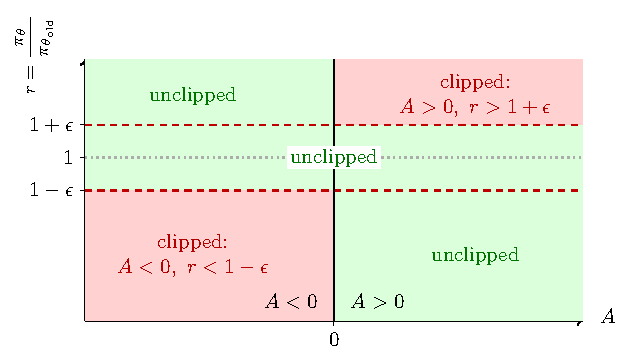
\includegraphics[width=0.7\linewidth]{figures/ppo_clip_region.pdf}
    \caption{PPO-Clip trust region in the $(A,r)$ plane, where $r=\pi_\theta(a|s)/\pi_{\theta_{\text{old}}}(a|s)$. The red region is the clipped region, and the green region is the unclipped region (after the clip and min operation).}
    \label{fig:ppo.clip.region}
\end{figure}

\textbf{Remark}
\begin{itemize}
    \item The popular choice of $\hat A_\phi(s_t,a_t)$ is $A^{\operatorname{GAE}(\gamma, \lambda)}_{\phi} = \sum_{\ell=0}^{T-1-t}(\gamma\lambda)^{\ell}\left(r_{t+\ell} + \gamma V^{\pi}_{\phi}(s_{t+1+\ell}) - V^{\pi}_{\phi}(s_{t+\ell}) \right)$.
    \item When $\hat A_\phi(s_t,a_t)>0$, which means that $a_t$ is better than the average, we want to increase its probability. However, we need to limit the increase to not being greater than the factor of $1+\epsilon$.
     \item When $\hat A_\phi(s_t,a_t)<0$, which means that $a_t$ is worse than the average, we want to decrease its probability. However, we need to limit the decrease to be no greater than the factor of $1-\epsilon$.
    
\end{itemize}

One can also constraint the distribution shift by
\begin{align}
     \max_{\theta} \Jcal_{\text{PPO-KL}}(\theta):= \Embb_{\tau\sim \pi_{\theta_{\text{old}}}}\left[ \sum_{t=0}^{T-1} \frac{\pi_{\theta}(a_t|s_t)}{\pi_{\theta_{\text{old}}}(a_t|s_t)} \hat  A_\phi(s_t,a_t) - \beta \operatorname{K L}\left[\pi_{\theta_{\text{old}}}(\cdot|s_t) || \pi_{\theta}(\cdot|s_t)\right]\right],
\end{align}

\textbf{Remark}
\begin{itemize}
    \item When maximize $\Jcal_{\text{PPO-KL}}(\theta)$, we minimize $\mathbb{D}_{K L}\left[\pi_{\theta_{\text{old}}}(\cdot|s_t)| | \pi_{\theta}(\cdot|s_t)\right]$, i.e., we minimize the forward KL, which has the \href{https://www.tuananhle.co.uk/notes/reverse-forward-kl.html}{mean-seeking behavior}.
\end{itemize}

% There's one missing piece though. How should we update the value (critic) network? Similar to objective funciton \eqref{eq:naive.critic.obj}, the $V^{\pi}_{\phi}$ can be updated by

% \begin{align}
%      \min \left\{\Lcal(\phi):= \Embb_{\tau\sim \pi_{\theta}}\left[ \sum_{t=0}^{T-1}(r_t+\gamma V^{\pi}_{\phi_{\text{old}}}(s_{t+1}) - V^{\pi}_{\phi}(s_t)\right]\right\}.
%      \label{eq:ppo.critic.obj},
% \end{align}
% where $V^{\pi}_{\phi_{\text{old}}}$ is the value network paired with $\pi_{\theta_{\text{old}}}$. There could be other variants for t

To put pieces together, we summarize the PPO-Clip in Algorithm~\ref{algo:ppo}.
\begin{algorithm}[H]
\caption{PPO-Clip Algorithm}
\begin{algorithmic}[1]
    \State Inputs: Initial Policy network parameter $\theta_0$ and value function parameter $\phi_0$.
    \For{k=0,1,2....}
        \State Collect a set of trajectories $D_k=\{\tau_n\}_{n=1}^{N}$.
        \State Reward-to-go calculation $G_t(\tau_n) = \sum_{t'=t}^{T_n-1}\gamma^{t'-t}r_{t'}$ for all $n$.
         \State GAE calculation $A^{\operatorname{GAE(\gamma,\lambda)}}_{\phi_k}(s_t^{(n)},a_t^{(n)})$ for all $t$ and $n$\footnote{Here $(s_t^{(n)},a_t^{(n)})$ means the state and action from t-step and n-th trajectory.}. 
        \State Approximately solve 
            \begin{align*}
                 \theta_{k+1}=\arg\max_{\theta} \frac{1}{N}\sum_{n=1}^{N}\frac{1}{T_n}
                  \sum_{t=0}^{T_n-1}  
                 \min\left\{\frac{\pi_{\theta}(a_t^{(n)}|s_t^{(n)})}{\pi_{\theta_{k}}(a_t^{(n)}|s_t^{(n)})}A^{\operatorname{GAE(\gamma,\lambda)}}_{\phi_k}(s_t^{(n)},a_t^{(n)}),  \right.
                 \\
                 \left.\operatorname{clip}\left(\frac{\pi_{\theta}(a_t|s_t)}{\pi_{\theta_{k}}(a_t|s_t)}, 1-\epsilon, 1+\epsilon\right)
                 A^{\operatorname{GAE(\gamma,\lambda)}}_{\phi_k}(s_t^{(n)},a_t^{(n)})\right\},
            \end{align*}
        \State Approximately solve 
            \begin{align*}
                \phi_{k+1}=\arg\min_{\phi} \frac{1}{N}\sum_{n=1}^{N}\frac{1}{T_n}
                  \sum_{t=0}^{T_n-1}(V^{\pi}_{\phi}(s_t^{(n)}) - G_t(\tau_n))^2
            \end{align*}
    \EndFor
\end{algorithmic}
\label{algo:ppo}
\end{algorithm}

\subsection{PPO in the context of RLHF}
Let us first introduce a new set of notions and setup. Let $\Dcal$ be a set of prompt and $x\in\Dcal$ is any sample from it. $y\sim \pi_{\theta}(\cdot|x)$ be a response sampled from the policy model $\pi_{\theta}$ given the prompt $x$. To simplify the discussion, let us assume that the reward model is given and we focus on the outcome reward $r(x,y)$. 

We consider the following variant objective function inspired by policy gradient and PPO
\begin{align*}
   \Jcal(\theta) = \Embb_{x\sim \Dcal, y\sim\pi_{\theta}(\cdot|x)} \left[ r(x,y) - \beta \operatorname{KL}\left[\pi_{\theta}(\cdot|x) || \pi_{\theta_{\text{ref}}}(\cdot|x)\right]\right],
\end{align*}
note that here we used forward KL divergence.
Then the gradient is 
\begin{align}\label{eq:RLHF.gradient.part1}
\grad \Jcal(\theta) = \int_{x\in \Xcal} p(x)\left\{\left[\int_{y\in\Ycal(x)}r(x,y)\frac{\partial}{\partial \theta}\pi_{\theta}(y|x)dy\right] - \beta \left[\int_{s\in\Ycal(x)}\frac{\partial}{\partial\theta}\pi_{\theta}(s|x)\log\frac{\pi_{\theta}(s|x)}{\pi_{\theta_{\text{ref}}}(y|x)}ds\right] \right\}dx,
\end{align}
where $\Xcal=\Dcal$ and $\Ycal(x)=\text{support}(\pi_{\theta}(y|x))$.
Note that
\begin{align}
    & \int_{s\in\Ycal(x)}\frac{\partial}{\partial\theta}\pi_{\theta}(s|x)\log\frac{\pi_{\theta}(s|x)}{\pi_{\theta_{\text{ref}}}(s|x)}ds  \nonumber\\
    & =  \int_{s\in\Ycal(x)}\left[\grad\pi_{\theta}(s|x)\cdot\log\frac{\pi_{\theta}(s|x)}{\pi_{\theta_{\text{ref}}}(s|x)} + \pi_{\theta}(s|x)\cdot \grad\log\frac{\pi_{\theta}(s|x)}{\pi_{\theta_{\text{ref}}}(s|x)}\right]ds \nonumber\\
    & = \int_{s\in\Ycal(x)}\left[\grad\pi_{\theta}(s|x)\cdot\log\frac{\pi_{\theta}(s|x)}{\pi_{\theta_{\text{ref}}}(s|x)} + \grad \pi_{\theta}(s|x)\right]ds \nonumber\\
    & = \int_{s\in\Ycal(x)}\grad\pi_{\theta}(s|x)\cdot\log\frac{\pi_{\theta}(s|x)}{\pi_{\theta_{\text{ref}}}(s|x)} ds \label{eq:RLHF.gradient.part2}
\end{align}  
where the last line follows from \eqref{eq:grad.log.prob}. Combining \eqref{eq:RLHF.gradient.part1} and \eqref{eq:RLHF.gradient.part2}, one obtains
\begin{align}\label{eq:RLHF.gradient.part3}
\grad \Jcal(\theta)
 & = \int_{x\in \Xcal} p(x)\left\{\left[\int_{y\in\Ycal(x)}r(x,y)\frac{\partial}{\partial \theta}\pi_{\theta}(y|x)dy\right] - \beta \left[\int_{s\in\Ycal(x)}\grad\pi_{\theta}(s|x)\cdot\log\frac{\pi_{\theta}(s|x)}{\pi_{\theta_{\text{ref}}}(s|x)} ds\right] \right\}dx \nonumber\\
 & = \int_{x\in \Xcal, y\in\Ycal(x)} p(x)\left\{ \pi_{\theta}(y|x) \left[ r(x,y)\grad\log \pi_{\theta}(y|x) - \beta\grad\log\pi_{\theta}(y|x)\cdot\log\frac{\pi_{\theta}(y|x)}{\pi_{\theta_{\text{ref}}}(y|x)}\right]  \right\}dydx \nonumber\\
 & = \Embb_{x\sim \Dcal, y\sim\pi_{\theta}(\cdot|x)}\left[\left(r(x,y) - \beta\log\frac{\pi_{\theta}(y|x)}{\pi_{\theta_{\text{ref}}}(y|x)}\right)\grad\log\pi_{\theta}(y|x)\right]
\end{align}
From \eqref{eq:RLHF.gradient.part3}, we conclude the "PPO" version of the RLHF objective function
\begin{align}\label{eq:rlhf.obj}
  \max_{\theta} \Jcal_{\text{RLHF}}(\theta):=\Embb_{x\sim \Dcal, y\sim\pi_{\theta}(\cdot|x)}\left[r(x,y) - \beta\log\frac{\pi_{\theta}(y|x)}{\pi_{\theta_{\text{ref}}}(y|x)}\right],
\end{align}
which recovers the first part of the objective function in Equation (2) of \citet{ouyang2022training}.